\section{Networking Layer} \label{sec:networking}

There are many devices on the Rubin summit network all of which must work in coordination to deliver smooth operations, hence reliability and scalability are important.
Following NIST \citep{NIST.SP.800-171} has also led us to some further segmentation ans isolation.
For automation all the networking configuration is Infrastructure as code using Ansible.

We also use software defined networking.
Originally this was with CISCO ACI but it proved complex, buggy and very proprietary.
We replaced all CISCO switches with Juniper and Arista devices.


\subsection{Reliability}

To make the summit operations secure and reliable the operational hardware is held in the \emph{pixel zone}
\figref{fig:pixel-zone}.
This isolates all operational machines with a 2FA VPN.
Device addresses and ports are restricted on all pixel zone machines ensuring we understand the traffic that
is supposed to be flowing and restricting any odd behavior.

\begin{figure}
\begin{centering}
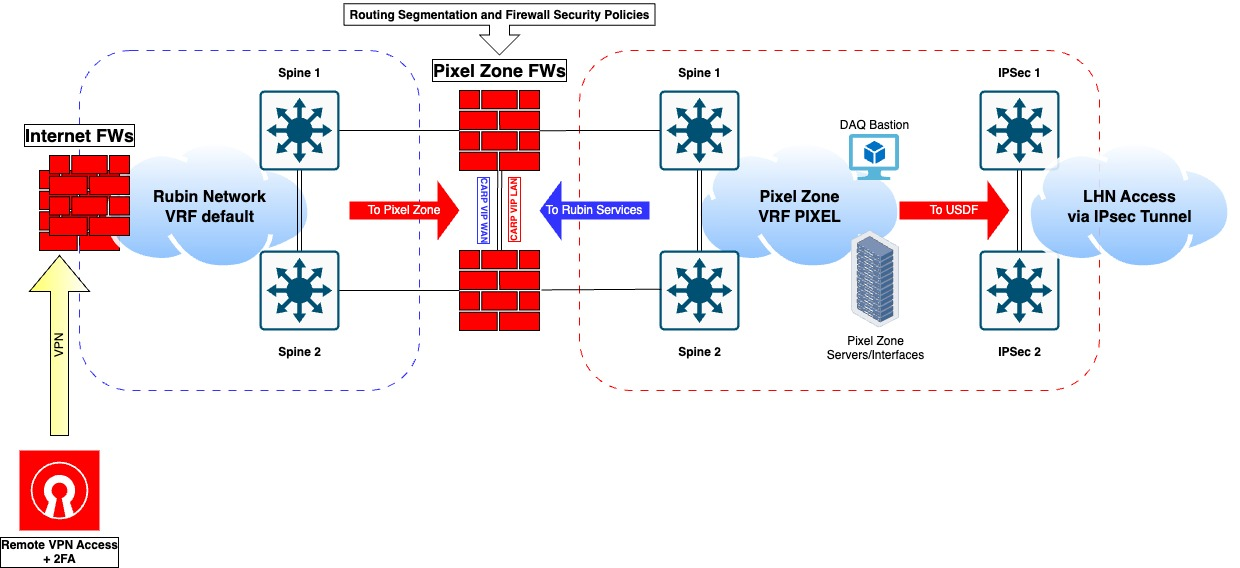
\includegraphics[width=0.9\textwidth]{images/pixel-zone}
        \caption{Rubin pixel zone to secure the summit
\label{fig:pixel-zone}}
\end{centering}
\end{figure}

\subsection{Scalability}
